\chapter{Environment}\label{chap:context}

\begin{sectionIntro}
    This chapter will describe essential facts about my internship, such as
    which company I did my internship at and what I worked on.
\end{sectionIntro}

\section{Company}

\subsection{Celad}
Celad is an IT consulting company with about 800 employees. It was created in Toulouse
and its headquarters are still in Toulouse.
The major activities of Celad cover:
\begin{description}
    \item [Information systems] such as solutions for E-banking, E-business, mobile applications.
    \item [Embedded sector] such as real-time, electronics, and aerospace.
\end{description}
One of its biggest clients in the embedded sector in Toulouse is Intel.
I did my internship as a contractor for Intel via Celad.

\subsection{Intel}
Intel Corporation is the world’s largest semiconductor chip maker. They
introduced the first microprocessor in 1971 and have been the world leader in
silicon innovation since.
Following a strategy to extend the Intel Architecture to new market segments,
they are delivering smartphones and tablets powered by Intel chipsets.

On figure \ref{fig:razri} below there is a picture of a smartphone with Intel inside.

\begin{figureGraphics}{Motorola Razr I with Intel inside}{fig:razri}
    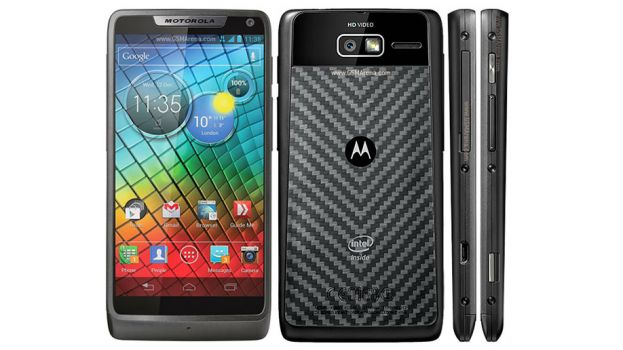
\includegraphics[width=\textwidth]{./src/img/razri.jpg}
\end{figureGraphics}

Some key figures of Intel:
\begin{itemize}
\item Leading manufacturer of computer, networking and communications
  products,
  \item 300 Facilities in 50 countries,
  \item Over \$35B in Annual Revenues from customers in over 120
    countries,
\item 23 Consecutive years of positive net income,
\item Approximately 80,000 employees,
\item 43,000 technical degrees, 12,000 Masters in Science, 4,000
  PhD’s, 4,000 MBA’s,
  \item One of the top ten most valuable brands in the world for 10
    consecutive years,
\item Invests \$100 Million each year in education across more than 50
  countries,
\item One of the top ten Linux \gls{kernel} contributors.
\end{itemize}


\subsection{Intel Audio feature team in Toulouse}
The team I worked with is the Audio feature team, in Toulouse.
They are responsible for the Audio \gls{hal} which is the interface between the
libraries and the \gls{android} \gls{kernel}. Intel made a custom Audio \gls{hal} to
replace \gls{android} default's one with their own one, which provides a lot more features.
The Intel Audio \gls{hal} is present in every \gls{android} device from 2011 or later with Intel inside, such
as the \emph{Motorola Razr I} from figure \ref{fig:razri}.

Their custom \gls{hal} is based around the \gls{pfw}, which will be described in the section \ref{sec:parameter-framework}.
TODO reorga the sections after this one.

\section{Android}
During my internship, I worked on the \gls{android} platform. This operating
system has a complex software stack which goes from the Linux \gls{kernel} to
applications such as \emph{Gmail}. This section gives an overview of the Android
stack to show on which components I worked.

\subsection{Global Android architecture}

The figure \ref{fig:archi} shows the Audio \gls{hal} which is between the
Linux \gls{kernel} and the libraries layers.
\begin{figureGraphics}{Global Android architecture}{fig:archi}
    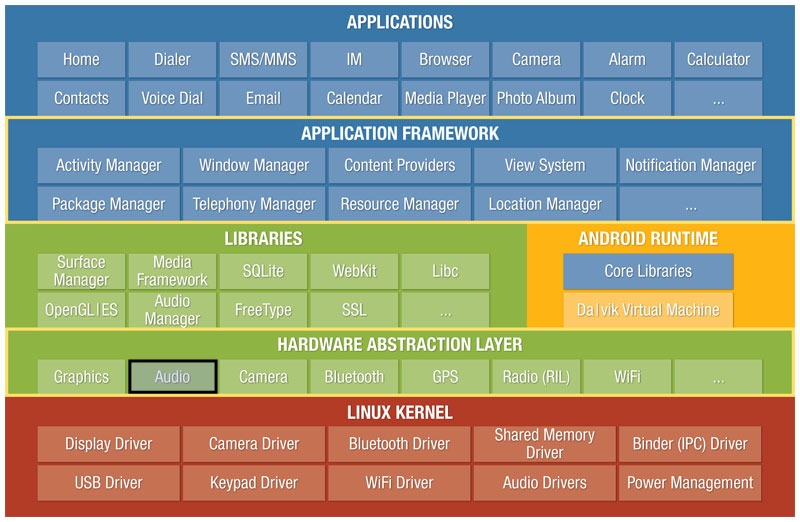
\includegraphics[width=\textwidth]{./src/img/android-archi-audio-hal.jpeg}
\end{figureGraphics}

Within the Audio feature team in Toulouse, we are mainly focused around the Audio \gls{hal}.

\subsection{Intel Audio HAL}
Intel's Audio \gls{hal} for Android platforms is based on a generic, plugin-based solution: the \gls{pfw}.
It runs in the \emph{userland}, which is easier to maintain than kernel-space code.
Since this solution is plugin-based, it is easy to extend and add more subsystems if needed.

There is an overview of the Intel Audio \gls{hal} on figure \ref{fig:hal} below.
\begin{figureGraphics}{Simplified view of Intel Audio HAL}{fig:hal}
    \includegraphics[height=0.5\textheight]{./src/img/hal-architecture.pdf}
\end{figureGraphics}
Two different instances of \gls{pfw} exist in the Intel Audio \gls{hal}:
\begin{description}
    \item[The route] \gls{pfw} communicates with the \emph{Stream Manager} and the \emph{Route Manager}.
        This side is responsible for translating events which come from upper layers into \emph{routes}, which
        is the concept understandable by the route manager.
    \item[The audio] \gls{pfw} communicates with the \emph{Route Manager} and the \gls{alsa} driver.
        This side talks to the drivers in order to set the different mixers in the correct state. For example,
        changing the gain of a mixer.
\end{description}

Some requirements of the Intel Audio \gls{hal}:
\begin{itemize}
    \item Since the audio system needs to be tuned by the tuning engineers, the \gls{hal} should be configurable.
        It would have been very painful to recompile the code at each time it is needed to adapt the value of a mixer!
    \item Since the \gls{hal} needs to \emph{abstract} the hardware variations, it should also be scalable. It should be
        easy to support new hardware.
\end{itemize}

The \gls{pfw} is a way to fulfill those requirements.

\section{Parameter-framework}
\label{sec:parameter-framework}
During a phone call, the smartphone isn't just transmitting the sound received from the microphone. Various algorithms are
applied on the audio signal which is transmitted and received.
On figure \ref{fig:audioArch} below we have an example of an audio architecture which shows the components involved.

\begin{figureGraphics}{Audio architecture of pandaboard}{fig:audioArch}
    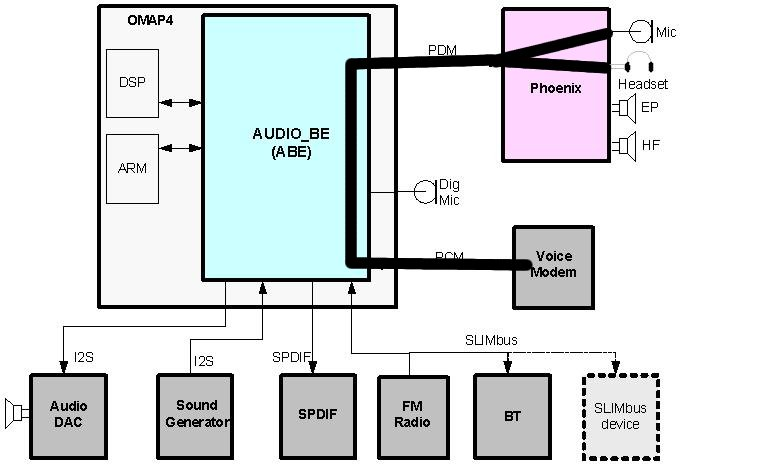
\includegraphics[height=0.5\textheight]{./src/img/Audio_arch2.jpg}
\end{figureGraphics}

The sound goes:
\begin{itemize}
    \item Trough the \emph{voice modem}
    \item Via the \emph{Audio Back End} where some voice processing algorithms (such as noise reduction) are applied
    \item Towards the \emph{Phoenix codec} to send the audio signal towards the headset.
\end{itemize}

Those algorithms have a lot of parameters, which can change depending on the use case: whether we are in a phone call,
or listening to some music. Furthermore, those parameters are \emph{often hardware dependent}.

The \gls{pfw} was designed to manage easily those multiple parameters in a scalable way.

\subsection{Some concepts}
In this section we are going to discover the concepts which make the
\gls{pfw} such a powerful tool.

\subsubsection{Structure}
The \gls{pfw} is first of all a hierarchical tree of parameters.
On figure \ref{fig:pfwtree} we can see an example of audio tree.

\begin{figureGraphics}{Parameter framework tree example}{fig:pfwtree}
    \fbox{\begin{minipage}{6cm}
            \dirtree{%
                .1 audio.
                    .2 microphone.
                        .3 echo\_cancellation.
                            .4 enable.
                            .4 configuration.
                                .5 gain.
                                .5 coefficient.
                    .2 speaker.
                        .3 equalizer.
                            .4 enable.
                            .4 configuration.
                                .5 filter.
                                .5 coefficient.
            }
    \end{minipage}}
\end{figureGraphics}

These structures are stored in \gls{xml} files. This is great because it implies that we don't need
to recompile the \gls{pfw} when changing the structure we are describing.

In listing \ref{lst:pfwstructure}, when can see the \gls{xml} structure file
describing the tree from figure \ref{fig:pfwtree}.

\begin{code}[language=pfwXml, caption=Structure file example snippet, label=lst:pfwstructure]
<!--snippet-->
<ComponentType Name="echo_cancellation">
    <BooleanParameter Name="enable"/>
    <ParameterBlock Name="configuration">
        <IntegerParameter Name="gain" Size="8"/>
        <IntegerParameter Name="coefficient" Size="8"/>
    </ParameterBlock>
</ComponentType>
<!--snippet-->
\end{code}

\subsubsection{Settings}
The \gls{pfw} is also able to change multiple parameters without any manual action, depending on the context.
The context is defined using a set of criteria. Those criteria are variables which can take a set of defined values.
For example, a criterion called \emph{Output Device} can take several values such as \emph{Speaker} or \emph{Headset}.

Depending on the value of those criteria, the \gls{pfw} can automatically apply a set of values towards
multiple parameters.
On listing \ref{lst:pfwsettings} we can see an example of setting file, written in a special language
which is translated into \gls{xml} by our build system.

\begin{code}[language=pfwLang, caption=Settings file example, label=lst:pfwsettings]
Domain:
    Conf: SpeakerWithEchoCancel
        OutputDevice Is Speaker
        Component: audio/speaker/
            echo_cancellation/enable = true
            configuration/gain = 2
            configuration/coefficient = 3
        # -- snippet --
    Conf: HeadsetWithEchoCancel
        OutputDevice Is Headset
        Component: audio/headset/
            echo_cancellation/enable = true
            configuration/gain = 3
            configuration/coefficient = 4 # arbitrary values
        # -- snippet --
\end{code}

\subsubsection{Extensibility}
Since the \gls{pfw} is \emph{plugin-based}, it is easy to extend its functionality to other usages than Audio, such
as Camera, or Bluetooth.


\subsection{Topic of my internship}
I worked within the Intel Audio development team, as an \emph{agile
software developer}. The team is customer oriented, using \gls{scrum}
methodology (see chapter \ref{chap:organisation}). My tasks
within the team were focused around enhancing and open-sourcing the \gls{pfw} on
\gls{GitHub}\footnote{see \ref{chap:annex}} to give the team some
visibility and advertise its work.
TODO explain this

\section{Workflow and environment}
In this section, we will cover my daily workflow. This helps
to understand how I proceeded during my whole internship.

\begin{figureGraphics}{Developer workflow}{fig:workflow}
    \includegraphics[height=0.6\textheight]{./src/img/workflow.pdf}
\end{figureGraphics}

This workflow is the same for every developer of the team. It is
detailed in the sub sections below.

\subsection{Development}
Android source tree contains more than 700 projects. They have their own build system
based on \lstinline{Android.mk} files. Each time that a project has to be rebuild from scratch (for example after a  \lstinline{make clean} command) all
the 700 projects of the Android source tree are scanned for dependencies. This requires a lot of computing power.
Given that fact, most of developers of our team are working on a remote server, via ssh.
The server we are connecting to is far more powerful than the desktops we use.
With its 32 cores and its 2 TeraBytes of SSD, compilation time was far less time-consuming
than compiling on my local machine (about 10 times faster).
This server also helps to have the same developer environment to avoid
time-consuming installations on local machines.

Working remotely on that server restrict developers to use command line programs only because
launching a graphical session for each user would require too much computing power.
During my internship, I sharpened my skills in \gls{vim} and discovered \gls{tmux}.
On the figure \ref{fig:setup} below, there is a screenshot of my development setup at Intel.

\begin{figureGraphics}{Development setup with vim and tmux}{fig:setup}
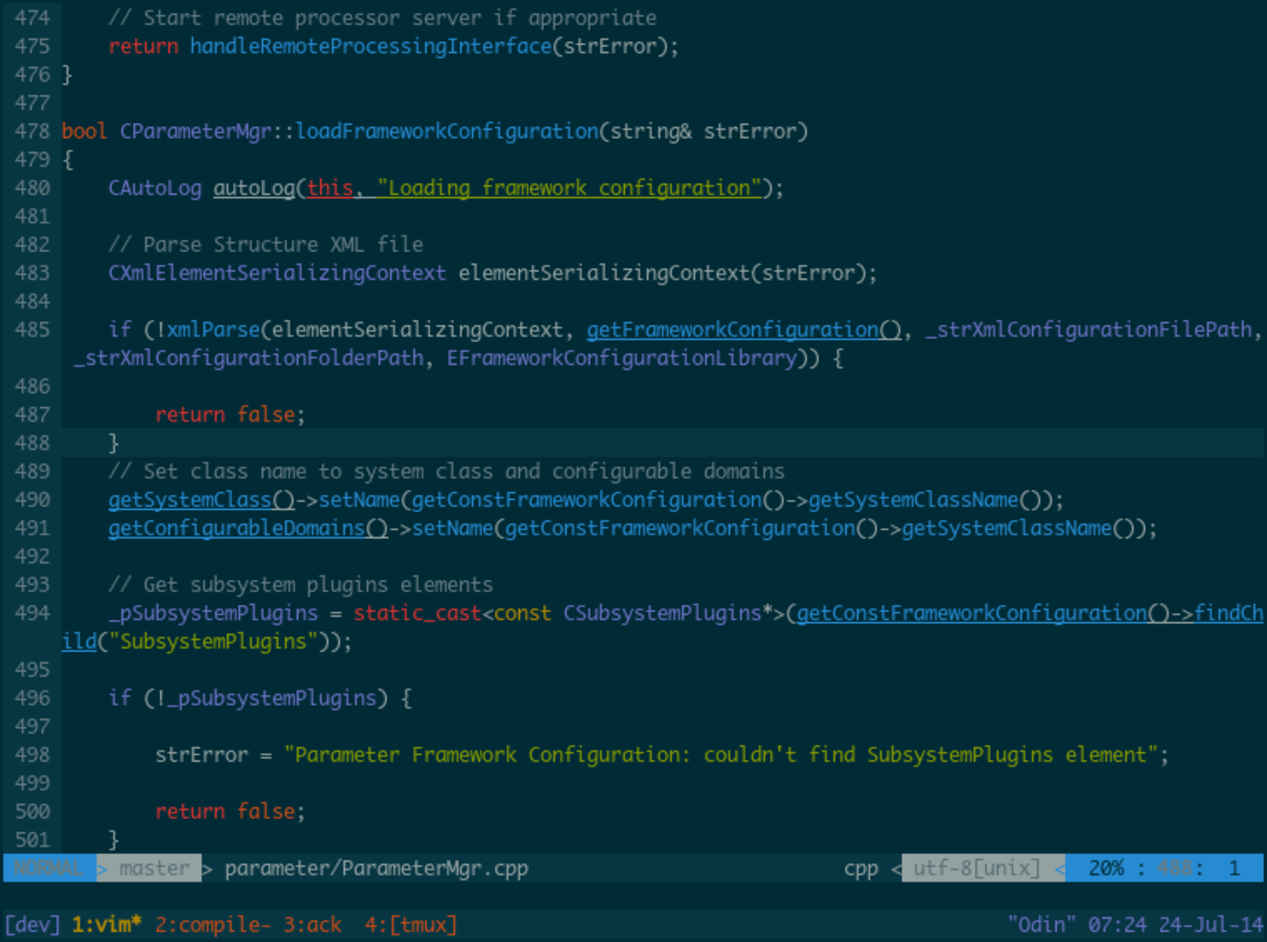
\includegraphics[width=\textwidth]{./src/img/setup.pdf}
\end{figureGraphics}

When the code is ready, I push it via \gls{git} on \gls{gerrit} to be reviewed.

\subsection{Git}
\gls{git} is a distributed revision control system initially designed for kernel
development. Given that fact, it can be used in environment which have large
code bases, such as \gls{android}. We use \gls{git} on daily basis at Intel for the
code delivered to customers and for the internal tools.

\subsection{Code quality}
Code quality matters. Clean code eases maintenance and is less error-prone.
Those facts are driving the team that I worked with at Intel. Naturally, all the
patches I have delivered during my internship have been reviewed and met the
expected quality.

Those reviews are done with the official \gls{android} review tool which is \gls{gerrit}.
It is based on a notation system with inline comments and its usage is pretty straightforward.
Its interface is showed on figure \ref{fig:gerrit} below.

\begin{figureGraphics}{Gerrit code review}{fig:gerrit}
    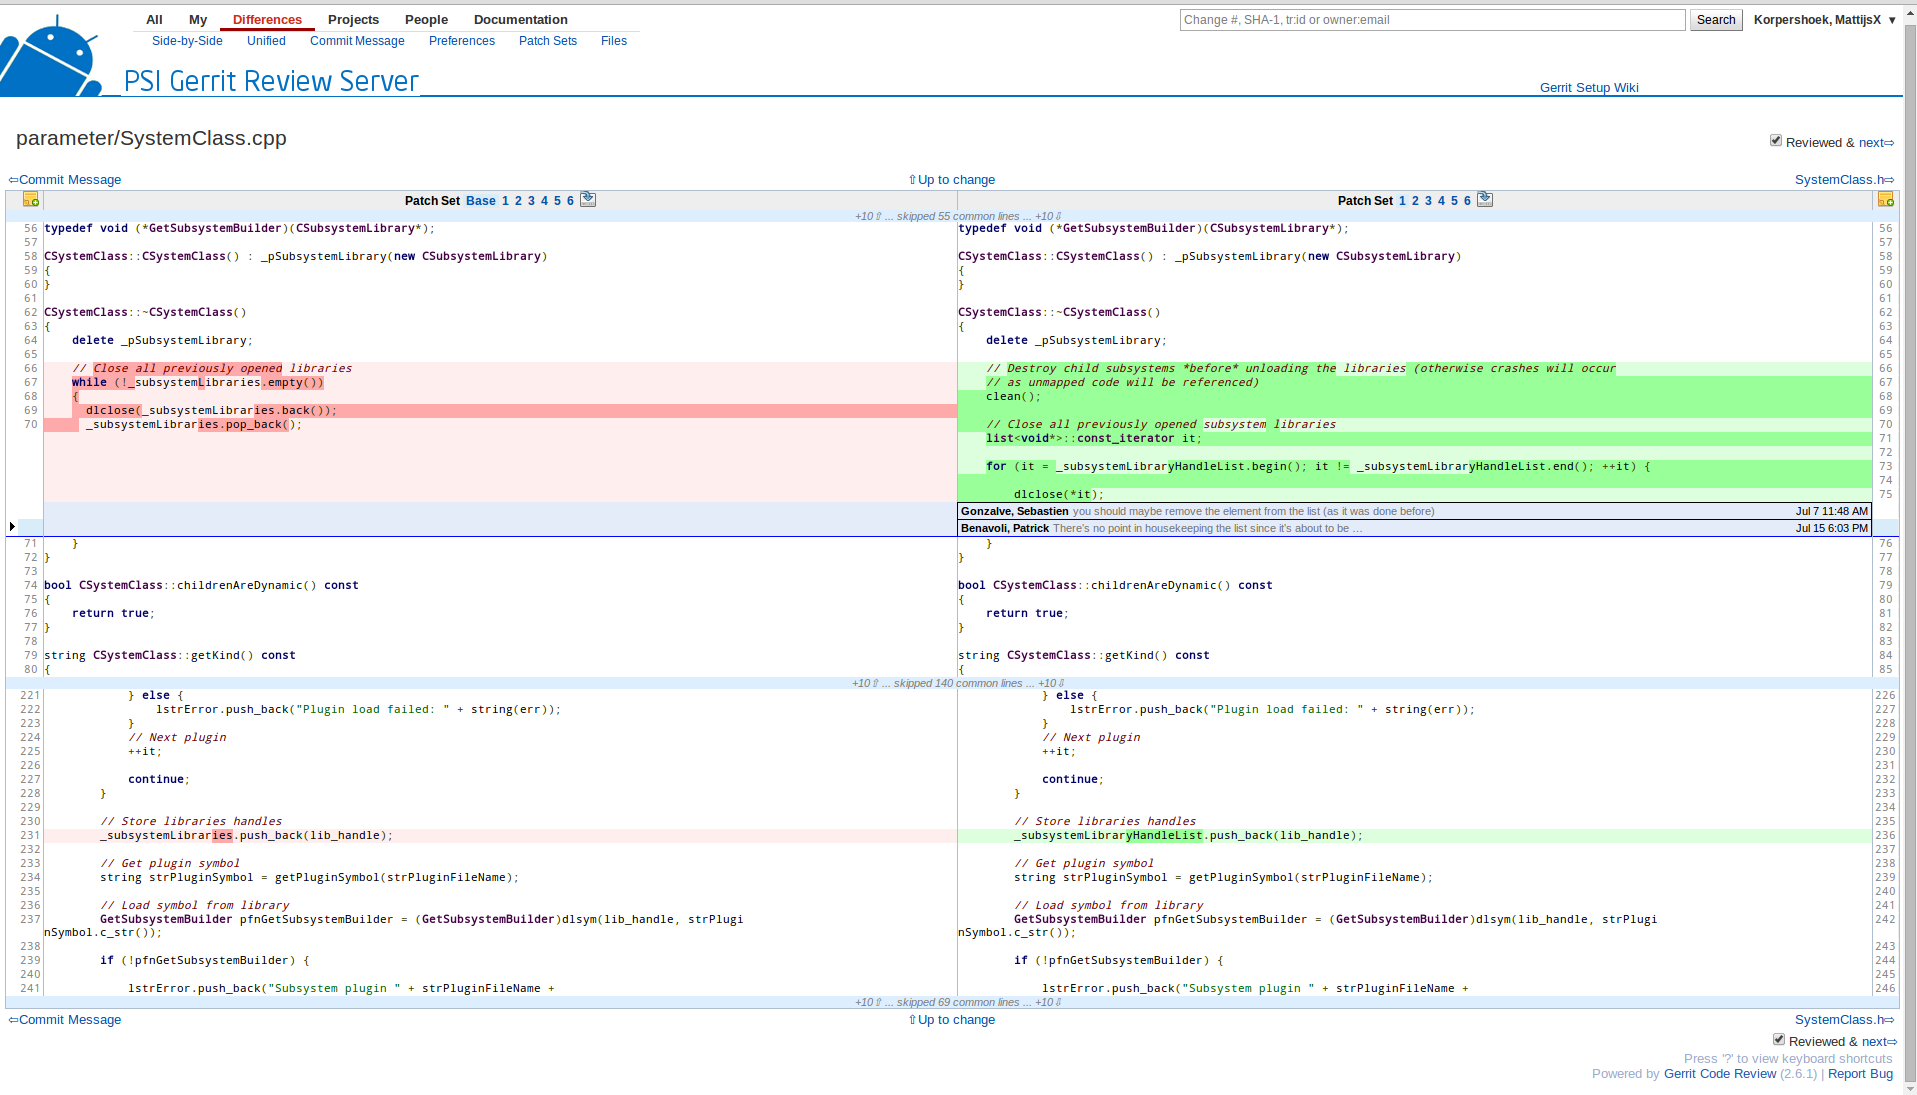
\includegraphics[width=\textwidth]{./src/img/gerrit.png}
\end{figureGraphics}

I have done some code review myself during this internship. It helps a lot to
understand how other people work. Viewing other peoples code also makes me come
up with new ideas to improve my own work in several aspects such as better naming,
more modularity, cleaner design.

\subsection{Submission to gatekeeping team}
After code review and a few reworks, the code is validated by the development team.
The super reviewer gives the developer the permission to submit his work to the gatekeeping team.
They are responsible for testing complex use cases and they ensure there is no regression nor side effects
due to the modifications the development team made.
A lot of automatic and manual tests scenarios are ran which cover \emph{voice call}, \emph{voip call}, \emph{media playback}
and more. Of course, more complex tests are done depending on the functionality which is developed.

